\pdfoutput=1
% \documentclass[conference]{IEEEtran}
% \documentclass[10pt, conference, letterpaper]{ IEEEtran}
% \IEEEoverridecommandlockouts
% \def\BibTeX{{\rm B\kern-.05em{\sc i\kern-.025em b}\kern-.08em
    % T\kern-.1667em\lower.7ex\hbox{E}\kern-.125emX}}
\documentclass[journal]{IEEEtran}
% \documentclass[journal,12pt,onecolumn,draftclsnofoot,]{IEEEtran}
\usepackage[utf8]{inputenc}
\usepackage{amsmath}
\usepackage{amsfonts}
\usepackage{bbding}
\usepackage{amssymb}
\usepackage{array}
\usepackage{multirow}
\usepackage{graphicx}
\usepackage[caption=false,font=footnotesize]{subfig}
\usepackage{algorithm}
\usepackage{algorithmic}
\usepackage[hidelinks]{hyperref}
\newcommand\algorithmicprocedure{\textbf{procedure}}
\newcommand{\algorithmicendprocedure}{\algorithmicend\ \algorithmicprocedure}
\makeatletter
\newcommand\PROCEDURE[3][default]{%
  \ALC@it
  \algorithmicprocedure\ \textsc{#2}(#3)%
  \ALC@com{#1}%
  \begin{ALC@prc}%
}
\newcommand\ENDPROCEDURE{%
  \end{ALC@prc}%
  \ifthenelse{\boolean{ALC@noend}}{}{%
    \ALC@it\algorithmicendprocedure
  }%
}
\newenvironment{ALC@prc}{\begin{ALC@g}}{\end{ALC@g}}
\makeatother

\usepackage{xcolor}
\usepackage{cite}

\allowdisplaybreaks
\renewcommand{\thefootnote}{\arabic{footnote}}
\DeclareMathOperator{\sgn}{\bf sgn}
\DeclareMathOperator{\cov}{\bf cov}
\DeclareMathOperator{\dom}{\bf dom}
\DeclareMathOperator{\var}{\bf var}
\DeclareMathOperator{\svd}{\bf svd}
\DeclareMathOperator{\expt}{\mathbb{E}}
\DeclareMathOperator{\vari}{\mathbb{V}}
\DeclareMathOperator{\proj}{\textrm{proj}}
\DeclareMathOperator{\gram}{\bf gram}
\DeclareMathOperator{\diag}{\bf diag}
\DeclareMathOperator{\Tr}{\bf Tr}
\DeclareMathOperator{\nsl}{\bf nsl}

\usepackage{amsthm}
\usepackage{stfloats}
\newtheorem{defi}{Definition}
\newtheorem{theorem}{Theorem}
\newtheorem{lemma}{Lemma}
\newtheorem{condition}{Condition}
\newtheorem{assumption}{Assumption}
\newtheorem{rem}{Remark}
\newtheorem{pro}{Property}
\newtheorem{prop}{Proposition}
\newtheorem{cor}{Corollary}
\newcommand{\blue}[1]{\textcolor{blue}{#1}}
\newcommand{\red}[1]{\textcolor{red}{#1}}
\newcommand{\violet}[1]{\textcolor{violet}{#1}}

\DeclareMathOperator*{\argmin}{\arg\!\min}
\DeclareMathOperator*{\argmax}{\arg\!\max}

\begin{document}
% \title{Lagrangian Dual for Joint Laser Link Matching and Traffic Flow Routing in Mega-Constellations}
% \title{\fontsize{21}{28}\selectfont Joint Laser Inter-Satellite Link Matching and Traffic Flow Routing in LEO Meta-Constellations: A Lagrangian Dual Approach}
\title{\fontsize{21}{28}\selectfont Joint Laser Inter-Satellite Link Matching and Traffic Flow Routing in LEO Mega-Constellations via Lagrangian Duality}

\author{
  \IEEEauthorblockN{Zhouyou Gu, Jihong Park, Jinho Choi}\\
\thanks{
Z. Gu and J. Park are with the Information Systems Technology and Design Pillar, Singapore University of Technology and Design, Singapore 487372 (email: \{zhouyou\_gu, jihong\_park\}@sutd.edu.sg).
}
\thanks{
J. Choi is with the School of Electrical and Mechanical Engineering,
the University of Adelaide, Adelaide, SA 5005, Australia
(email: \{jinho.choi\}@adelaide.edu.au).
}% \IEEEauthorblockA{\textit{dept. name of organization (of Aff.)} \\
% email address}\\
\thanks{Source codes will be available upon acceptance.}
% \vspace{-1.25cm}
}

\maketitle

\begin{abstract}
Low Earth orbit (LEO) mega-constellations greatly extend the coverage and resilience of future wireless systems. Within the mega-constellations, laser inter-satellite links (LISLs) enable high-capacity, long-range connectivity. Existing LISL schemes often overlook mechanical limitations of laser communication terminals (LCTs) and non-uniform global traffic profiles caused by uneven user and gateway distributions, leading to suboptimal throughput and underused LCTs/LISLs -- especially when each satellite carries only a few LCTs. This paper investigates the joint optimization of LCT connections and traffic routing to maximize the constellation throughput, considering the realistic LCT mechanics and the global traffic profile. The problem is formulated as an NP-hard mixed-integer program coupling LCT connections with flow-rate variables under link capacity constraints. Due to its intractability, we resort to relaxing the coupling constraints via Lagrangian duality, decomposing the problem into a weighted graph-matching for LCT connections, weighted shortest-path routing tasks, and a linear program for rate allocation. Here, Lagrange multipliers reflect congestion weights between satellites, jointly guiding the matching, routing, and rate allocation. Subgradient descent optimizes the multipliers, with provable convergence. Simulations using real-world constellation and terrestrial data show that our methods substantially improve network throughput by up to $35\%$--$145\%$ over existing non-joint approaches.
\end{abstract}

\begin{IEEEkeywords} 
Mega-constellations; Laser links; Graph theory.
\end{IEEEkeywords}


\section{Introduction}
Low Earth orbit (LEO) satellites are emerging as a cornerstone of future generations of wireless communication systems, particularly in providing ubiquitous connectivity worldwide \cite{maiolinicapez2024use}.
Owing to their reduced propagation delays and improved link budgets to terrestrial terminals, the deployment of LEO satellite constellations complements terrestrial networks and extends the network coverage by enabling direct connections to users \cite{he2024directtosmartphone}.
Commercial proprietary programs such as SpaceX’s Starlink and OneWeb have been deploying thousands of LEO satellites, forming mega-constellations \cite{wu2025enhancing}.
The integration of laser inter-satellite links (LISL) using free-space optical (FSO) systems in the LEO mega-constellations promises to deliver high data rates and long ranges in inter-satellite communications \cite{elamassie2023freea}, connecting the traffic flows across the whole constellation.

Compared to radio frequency (RF) links, LISLs modulate data using directional beams that emit nearly all the transmitted energy into a narrow path, thereby minimizing energy spreading \cite{ntontin2025vision}. 
However, due to the narrow beam width, one laser communication terminal (LCT) can only connect to one other LCT at a time, limiting the number of LISLs that can be established \cite{wang2024free}. 
Also, the beam steering is subject to mechanical limitations such as limited steering range and vibrations, which can further restrict the connectivity of the constellation \cite{kaymak2018survey}.
Thus, how to allocate the scarce LCTs to maximize the constellation connectivity while considering their mechanical limitations is a critical challenge.

Given the limited LCT resources on each satellite, simple designs use grid patterns that link each satellite to its immediate neighbors in the same orbital plane and to satellites in adjacent planes \cite{chaudhry2021laser,chen2021analysis}.
In this approach, the offset of the connected LCTs between adjacent orbital planes can be further adjusted to optimize the constellation connectivity \cite{rao2025minimumhop,guo2024constellation}.
Alternatively, the authors in \cite{bhattacherjee2019network} propose connecting the LISLs via optimized motifs (small, repeated connection patterns).
More flexible designs use maximum weight matching (MWM) that assigns weights to all potential LISLs and connects the LCTs based on these weights \cite{leyva-mayorga2021interplane,ron2025time}. Here, weights are assigned based on a single LISL property, e.g., maximum link rate \cite{leyva-mayorga2021interplane}, or a score that considers multiple link characteristics, e.g., capacity and latency \cite{ron2025time}.
However, these designs ignore the diverse traffic profiles across the constellation due to the uneven distribution of users and gateways.
This can lead to underutilized LCTs and LISLs and suboptimal network throughput \cite{bhattacherjee2019network}. 
Incorporating traffic flow routing into the LCT connection design is essential to improve the overall throughput of the constellation.

Jointly optimizing the link connections and traffic routing in a network is a well-known mixed-integer programming problem that is NP-hard \cite{ahuja1993network}.
One powerful technique to solve the problem efficiently is to use Lagrangian duality \cite{fisher2004lagrangian}.
It views the integer program as a core problem plus a set of complicating constraints, and by lifting these constraints to the objective function with Lagrange multipliers (or Lagrangian dual variables), the original problem is relaxed and can be solved efficiently due to fewer constraints \cite{ahuja1993network}. 
This method has been successfully applied to optimize the network coding multicast rates \cite{wang2023joint} and per traffic flow's energy efficiency  \cite{huang2025lagrangianbased} in satellite networks by lifting bottleneck link constraints and end-to-end path length constraints, respectively.
Nevertheless, how to design the Lagrangian dual method for considering practical LCT mechanical limitations and global traffic profiles in LEO mega-constellations is still an open question.



\begin{table*}[t]
  \centering
  \caption{Summary of Notations}
  \label{tab:notation}
  \vspace{-0.15cm}
  \footnotesize
  \setlength{\tabcolsep}{4pt}
  \renewcommand{\arraystretch}{1.05}
  \begin{tabular}{@{}l p{0.35\textwidth} l p{0.35\textwidth}@{}}
    \hline
    \textbf{Symbol} & \textbf{Definition} & \textbf{Symbol} & \textbf{Definition} \\
    \hline
    $t$ & System time (s) & $\mathcal{T}_0$ & Real-world reference time at $t=0$ \\

    $I$, $\mathcal{I}$ & Number of satellites; set of satellites & $\mathbf{l}_i(t)$, $\mathbf{v}_i(t)$ & Position and velocity of satellite $i$ in ECI (m, m/s) \\

    $z_{i,j}(t)$ & Distance between satellites $i$ and $j$ (m) & $\mathbf{d}_{i,j}(t)$ & Unit direction vector from $i$ to $j$ \\

    $N'$ & Number of LCTs per satellite & $N,\ \mathcal{N}$ & Total number of LCTs; set of all LCTs \\

    $i_n$ & Satellite index that LCT $n$ belongs to & $\mathbf{u}_n$ & Mounting direction of LCT $n$ (unit vector) \\

    $\theta$ & LCT field-of-regard (FOR) half-angle (rad) & $\nu$ & Pointing jitter angle (rad) \\

    $\sigma_{\mathrm{J}}$ & Rayleigh scale parameter of pointing jitter & $P_0$ & Optical transmit power (W) \\

    $\Phi(y,z)$ & Gaussian beam intensity at $(y,z)$ & $\Phi_0$ & Peak intensity at beam waist \\

    $W_0$ & Beam waist radius (m) & $W(z)$ & Beam radius at distance $z$ \\

    $z_{\mathrm{R}}$ & Rayleigh range & $C(y,z)$ & LISL capacity lower bound (bps) \\

    $B$ & Receiver bandwidth (Hz) & $A$ & LCT aperture area (m$^2$) \\

    $\Psi$ & Receiver responsivity (A/W) & $\sigma_{\mathrm{N}}$ & Noise amplitude (A) \\

    $U_i(t)$ & Number of Users covered by satellite $i$ & $D$ & Per-user traffic demand (Gbps) \\

    $Q$ & Gateway capacity per satellite (Gbps) & $Q_i(t)$ & Serving rate of satellite $i$ (Gbps) \\

    $D_i(t)$ & Demand rate of satellite $i$ (Gbps) & $\mathcal{G}^{\text{LCT}}=(\mathcal{N},\mathcal{E})$ & LCT connectability graph \\

    $\hat{z}$ & Max distance for connectable LCT pair & $\mathcal{E}$ & Set of connectable LCT pairs \\

    $c_{n,m}$ & LISL establishment indicator between LCTs $n$ and $m$ & $\mathcal{C}$ & Feasible set of LCT connections $\mathbf{c}$ \\

    $M$ & Number of nearest serving satellites considered & $\mathcal{F}$ & Set of traffic source--target satellite pairs $(s,s')$ \\

    $q^{s,s'}$ & Flow rate from $s$ to $s'$ (Gbps) & $\mathbf{q},\ \mathcal{Q}$ & Flow vector and its feasible set \\

    $\mathcal{E}_{i,j}$ & Connectable LCT pairs between sats $i$ and $j$ & $\mathcal{L}$ & Neighboring satellite pairs (potential links) \\

    $\mathcal{G}^{\text{SAT}}=(\mathcal{I},\mathcal{L})$ & Satellite connectivity graph & $x^{s,s'}_{i,j}$ & Routing indicator of flow $(s,s')$ on link $(i,j)$ \\

    $\mathbf{x},\ \mathcal{X}$ & Routing decisions and feasible set & $r_{n,m}$ & Effective LISL data rate of LCT pair $\{n,m\}$ \\

    $\epsilon$ & LISL outage probability threshold & $\lambda_{i,j}$ & Lagrange multiplier for link-rate constraint on $(i,j)$ \\
    \hline
  \end{tabular}
  \vspace{-0.25cm}
\end{table*}


This paper investigates the joint optimization of LISL matching and traffic flow routing in LEO mega-constellations, where the objective is to maximize the network throughput routed through the established LISLs. We first formulate the joint problem based on the models of constellation orbits, LCT mechanics and traffic profiles.
To solve this NP-hard problem, we apply the Lagrangian dual relaxation method by lifting the maximum rate limitation constraints between neighboring satellites via Lagrange multipliers.
Each Lagrange multiplier represents the congestion level of a satellite pair: a larger multiplier indicates that matching the pair's LCTs addresses higher traffic demands, Conversely, it also indicates that the LISLs are more congested and should be avoided in routing.
This effectively decouples the joint problem into three Lagrange multiplier-weighted subproblems: a) a weighted graph matching problem for LCT pairs, b) a weighted shortest-path routing problem for each traffic flow, and c) a linear program (LP) maximizing the network throughput.
Based on this fact, we can jointly optimize the LISL matching and flow routing decisions by adjusting the multipliers, e.g., via the subgradient descent \cite{boyd2003subgradient}.
Our contributions are summarized as
\begin{itemize}
  \item We provide a comprehensive formulation of the problem \eqref{eq:prob:constrainted_routing_and_matching:primal}, including the LCTs' steering ranges and vibrations, and the diverse traffic profile across the constellation.
  \item We relax the link rate limitation constraints of satellite pairs in \eqref{eq:prob:constrainted_routing_and_matching:relaxed} and  \eqref{eq:prob:constrainted_routing_and_matching:dual}, separating the original problem into subproblems (i.e., (a), (b), and (c) in \eqref{eq:prob:constrainted_routing_and_matching:lagrangian_dual}) that are solved independently at polynomial complexity.
  \item Building on this, we design a Lagrangian dual-based subgradient-descent algorithm (\textbf{DuJo}) and prove that the set of optimal Lagrange multipliers and the subgradient are bounded, guaranteeing the convergence of the algorithm to the optimal multipliers (\textbf{Theorem} \ref{theorem:convergence:classic}).
  \item With simulations based on real-world constellation and terrestrial information, we show that our method \textbf{DuJo} can improve the network throughput in Starlink-based constellations approximately by up to $145\%$ compared to a grid-aligned LISL scheme and up to $35\%$ compared to a scheme prioritizing high-capacity LISLs.
\end{itemize}

\subsection{Notations and Paper Organization} 
The $i$-th element of a vector $\mathbf{x}$ is denoted as $x_{i}$.
The $j$-th element of the $i$-th row of a matrix $\mathbf{x}$ is denoted as $x_{i,j}$.
Table \ref{tab:notation} summarizes the notations used in this paper.
We collect all the elements in $\mathbf{x}$ as $\{x_{i,j}\}_{\forall(i,j)}$.
The rest of this paper is organized as follows. Section \ref{sec:system_model} presents the system model of the LEO mega-constellation, the models of LCT mechanics and traffic profiles.
Section \ref{sec:problem_formulation} formulates the constellation graphs and the joint optimization problem over the graphs, and Section \ref{sec:lagrangian_dual_relaxation} presents the Lagrangian dual relaxation of the joint problem.
Section \ref{sec:simulation} shows the simulations evaluating the proposed methods, and Section \ref{sec:conclusion} concludes this work.




\section{System Model of Mega-Constellation}\label{sec:system_model}
This section explains the system model of the mega-constellation connected by LISLs, as illustrated in Fig. \ref{fig:leo_system_diagram}.

\subsection{Constellation Model}

The time of the system is denoted by $t$ in seconds, where $t=0$ is the initial time corresponding to a real-world time $\mathcal{T}_0$. 
The spatial domain is described in Cartesian coordinates, with the origin fixed at the center of the Earth \cite{vallado2022fundamentals}.
The satellites and the Earth are assumed to move with respect to the Earth-centered inertial (ECI) frame.
In the ECI frame, the direction of the vernal equinox is taken as the reference direction along the x-axis, and the z-axis is aligned with the Earth's rotation axis. The Earth rotates about the z-axis at an angular velocity of $7.2921 \times 10^{-5}$ rad/s. The Earth's radius is set to $6.3781 \times 10^6$ m.
We consider a mega-constellation with $I$ satellites that are collectively denoted as $\mathcal{I} = \{1,\dots,I\}$.
Each satellite has a near-circular orbit described by two-line element sets (TLEs).
The position and the velocity of satellite $i \in \mathcal{I}$ at time $t$ is denoted by $\mathbf{l}_i(t)$ (m) and $\mathbf{v}_i(t)$ (m/s) in the ECI frame, respectively, which is determined by the TLEs.
The distance and direction vector from satellite $i$ to $j$ are denoted by $z_{i,j}(t)$ and $\mathbf{d}_{i,j}(t)$, respectively, which are given by
\begin{equation}
  \begin{aligned}
    z_{i,j}(t) = \|\mathbf{l}_i(t) - \mathbf{l}_j(t)\|\ 
    \text{and}\ 
    \mathbf{d}_{i,j}(t) = \frac{\mathbf{l}_j(t) - \mathbf{l}_i(t)}{z_{i,j}(t)}.
  \end{aligned}
\end{equation}

\subsection{Satellite Form Factor and LCT Mechanics Models}
We model each satellite as a rigid body that can rotate in space by using its attitude control system \cite{vallado2022fundamentals}.
The satellites maintain their orientations and their body frames always pointing to the center of the Earth, i.e., in the direction of $-\mathbf{l}_i(t)$ at time $t$.
Each satellite $i$ is equipped with $N'$ LISL communication transceivers (LCTs), and there are total $N$ LCTs in the constellation, i.e., $N=N'I$. We denote the set of all LCTs as $\mathcal{N} = \{1,\dots,N\}$.
We write the index of the satellite that LCT $n$ belongs to as $i_n$, where $i_n \in \{1,\dots,I\}$. 
LCT $n$ has a mounting direction $\mathbf{u}_n(t)$ in the ECI frame, which is a unit vector fixed on the satellite body.
Each LCT can steer its beam to point at any direction with an angle less than $\theta$ in radians from its center mounting direction, e.g., using steering mirrors. Here, this region is referred to as its field of regard (FOR).
Due to space dynamic and satellite motion, the beam pointing direction of the LCT can be deviated from the desired direction randomly with small unpredictable errors, referred to as pointing jitters.
The pointing jitter in radians is assumed to follow a Rayleigh distribution \cite{arnon2003effects} as
\begin{equation}\label{eq:pointing_jitter}
  \begin{aligned}
    f_{\text{jitter}}(\nu) = \frac{\nu}{\sigma^2_{\mathrm{J}}} \exp\left(-\frac{\nu^2}{2\sigma^2_{\mathrm{J}}}\right), \nu \geq 0.
  \end{aligned}
\end{equation}
Furthermore, the pointing error is assumed to be independent and identically distributed (i.i.d.) for each LCT.

\subsection{LCT Beam Model}
Laser beams are modeled as Gaussian beams \cite{saleh2019fundamentalsa}. 
Each beam is configured with power $P_0$ watts (W).
The intensity of a propagating Gaussian beam is given by
\begin{equation}
  \begin{aligned}
\Phi(y,z)=\Phi_0\left(\frac{W_0}{W(z)}\right)^2 \exp\!\left(-\frac{2y^2}{W(z)^2}\right),
  \end{aligned}
\end{equation}
where $\Phi_0$ is the intensity at the center of the beam at the beam waist, $y$ is the radial distance from the beam's center and $W(z)$ is the beam radius at distance $z$ from the beam waist and $W_0$ is the beam waist radius.
Here, the peak intensity $\Phi_0$ and the beam radius $W(z)$ are modeled as
\begin{equation}
  \begin{aligned}
    \Phi_0 = \frac{2P_0}{\pi W_0^2}, \
    W(z)=W_0\sqrt{1+\left(\frac{z}{z_\mathrm{R}}\right)^2},
  \end{aligned}
\end{equation}
where $z_\mathrm{R}$ is the Rayleigh range of the beam.
The data in LISLs is transmitted using an intensity-modulation and direct-detection scheme, e.g., ON-OFF keying (OOK). While the closed-form expression for the channel capacity cannot be derived, the lower bounds on the capacity have been studied.
Specifically, given $y$ and $z$, the channel capacity of the LISL is lower bounded as \cite{farid2007outage,lapidoth2009capacity,chaaban2022capacity}
\begin{equation}
  \begin{aligned}
    C(y,z) \approx \frac{B}{2}\log_2
    \left(1+\frac{\left( A \cdot \Phi(y,z)\cdot \Psi  \right)^2}{2\pi e \sigma^2_{\mathrm{N}}} \right),
  \end{aligned}
\end{equation}
where the unit is in bits per second (bps), $\Psi$ is the LCT receiving optical sensor's responsivity in ampere/watt (A/W), $B$ is the bandwidth of the receiver in Hertz (Hz), $A$ is the aperture area of the LCTs in m$^2$, and $\sigma_{\mathrm{N}}$ is the noise amplitude in ampere (A) \cite{maxim_spf_transimpedance}.
For sufficiently small pointing jitter angles, the radial distance $y$ can be approximated as $y \approx z \nu$. 
The capacity of the LISL, as a function of the pointing jitter $\nu$ and the satellite distance $z$, can be written as $C(z \nu,z)$. We assume ideal acquisition and tracking processes of the LCTs, i.e., there are no acquisition time losses and no additional tracking errors.

%The capacity of the LISL can be written in terms of the pointing jitter and the satellite distance as $\nu$ as $C(z\nu,z)$. We assume the acquisition and tracking processes of the LCTs are ideal, i.e., there are no acquisition time and additional tracking errors.

\begin{figure}[t]
  \centering
  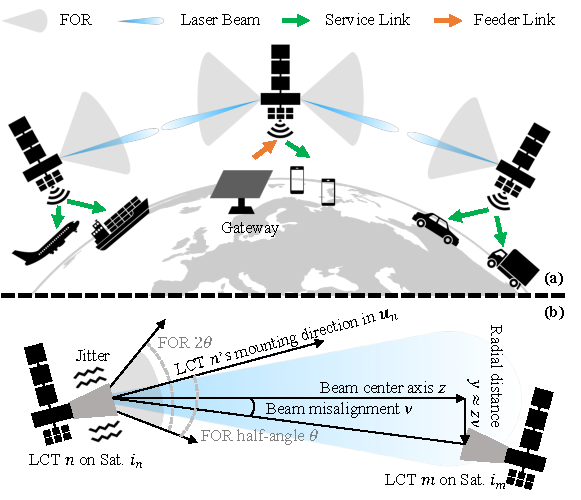
\includegraphics[scale=0.9]{leo_system_diagram.pdf}
  \vspace{-0.2cm}
  \caption{Illustration of a) the LEO satellite mega-constellation, and b) the LCT and beam model from one LCT to another.}
  \label{fig:leo_system_diagram}
  \vspace{-0.25cm}
\end{figure}



\subsection{Traffic Profile Model}

As the focus of this paper is on the LCT management in space, we consider a simplified scenario where the constellation is serving the traffic from gateways to users under its coverage over the globe.

It is assumed that each user is downloading data from the Internet, e.g., for video streaming via the service links. We assume that each satellite $i$ has a random number of users, denoted by $U_i(t)$, within its coverage area at time $t$, and each user has a traffic demand of $D$ Gbps.
We consider there are multiple ground gateways scattered on the Earth, and each satellite can serve up to $Q$ Gbps of traffic if a ground gateway lies within its coverage area. 
Note that with a ground gateway connection, a satellite can not only serve traffic demands of the users under its coverage but also from other satellites in the constellation when they are connected by LISLs.
Each satellite first serves the traffic demand of its own users under its coverage, i.e., $U_i(t) D$ Gbps for satellite $i$, and then serves the traffic demand of other satellites by using its remaining gateway capacity.
Specifically, by subtracting the traffic demand of the users under its own coverage, each satellite $i$ can serve the traffic demand of other satellites up to
\begin{equation}
  \begin{aligned}
    Q_i(t) = \begin{cases}
      (Q - U_i(t) D)_{+},\ &\text{if satellite $i$ has a gateway},\\
      0,\ &\text{otherwise},
    \end{cases}    
  \end{aligned}
\end{equation}
which is referred to as the traffic serving rate of satellite $i$ to the constellation. Here, $(x)_{+} = \max\{x,0\}$. 
Similarly, the traffic demand of satellite $i$ is the remaining part of the traffic demand of the users under its coverage that is not served by its own gateway connection (if it has one) and is denoted as 
\begin{equation}
  \begin{aligned}
    D_i(t) = \begin{cases}
      (U_i(t) D-Q)_{+},\ &\text{if satellite $i$ has a gateway},\\
      U_i (t)D,\ &\text{otherwise},
    \end{cases}    
  \end{aligned}
\end{equation}
which is referred to as the traffic demand rate of satellite $i$ to the constellation.
Here, positive traffic demand of a satellite needs to be served by other satellites with a ground gateway connection via the LISLs.
Satellites with positive serving or positive demanding rates are referred to as serving and demanding satellites, respectively.

\section{Problem Formulation}\label{sec:problem_formulation}
We consider the constellation at a given time $t$, where we omit $t$ for simplicity for the rest of the paper. 
The task is to maximize the network throughput in the constellation by optimizing 1) the connecting pairs of LCTs, 2) the traffic flow allocation between serving and demanding satellites, and 3) the routing of the traffic flows through the established LISLs.
To construct the problem, we first define three independent feasible domains constraining the above groups of decision variables, and then formulate the maximum link rate limitation constraints that couple these decision variables.

\subsection{LCT Connection Constraints}
The LCTs $\mathcal{N}$ and all connectable LCT pairs $\mathcal{E}$ are modeled as a graph $\mathcal{G}^\text{LCT} = (\mathcal{N},\mathcal{E})$, where the vertices are the LCTs and the edges are connectable LCT pairs.
A potential LISL can be established between a pair of LCTs only if the distance between the satellites on which the LCTs are mounted is less than a maximum beam transmission distance $\hat{z}$ and their satellites are in the FOR of each other.
Mathematically, the set $\mathcal{E}$ of all connectable LCT pairs is expressed as
\begin{equation}
  \begin{aligned}
    &\mathcal{E} = \big\{\{n,m\}\ \big| \ i_n \neq i_m, z_{i_n,i_m} \leq \hat{z}, \\
    &\qquad\qquad \mathbf{d}_{i_n,i_m} \cdot \mathbf{u}_n > \cos \theta,\mathbf{d}_{i_m,i_n} \cdot \mathbf{u}_m > \cos \theta \big\}.
  \end{aligned}
\end{equation}
Denote by $c_{n,m}$ the binary indicator on whether the LISL from LCT $n$ to $m$ is established or not. If the LISL is established from LCT $n$ to $m$, it is also established from LCT $m$ to $n$, which can be mathematically expressed as
\begin{equation}\label{eq:const:link:binary_bidirectional_connection}
  \begin{aligned}
    c_{n,m}\in \{0,1\},\ c_{n,m} = c_{m,n} ,\ \forall n\neq m.
  \end{aligned}
\end{equation}
Each LCT can only connect to one other LCT at a time, i.e., 
\begin{equation}\label{eq:const:link:one_connection}
  \begin{aligned}
    \sum_{m\in\mathcal{N}} c_{n,m} = 1,\ \forall n\in\mathcal{N}.
  \end{aligned}
\end{equation}
By collecting indicators $c_{n,m}$ as a vector  $\mathbf{c} = \{c_{n,m}\}_{(n,m)\in\mathcal{E}}$, the feasible domain of LCT connections is defined as
\begin{equation}
  \begin{aligned}
    \mathcal{C} = \left\{ \mathbf{c} \ \big|\   \eqref{eq:const:link:binary_bidirectional_connection},\eqref{eq:const:link:one_connection}\right\}.
  \end{aligned}
\end{equation}


\subsection{Traffic Serving and Demand Rates Constraints}
When there is no restriction, a demanding satellite $s'$ can be served by any satellite with a ground gateway connection. This will lead to a significant number of traffic source-target pairs, increasing the problem complexity.
To reduce the traffic source-target satellite pairs, we assume that a demanding satellite $s'$ can only be served by its $M$ nearest satellites via LISLs.
We denote the $M$-nearest satellites with ability to serve traffic for satellite $s'$ as $\mathrm{TopM}_{s:Q_s > 0} -z_{s,s'}$, where $z_{s,s'}$ is the distance from satellite $s$ to $s'$.
We collect all the traffic source and target satellite pairs in a set $\mathcal{F}$ as
\begin{equation}
  \begin{aligned}
    \mathcal{F} = \{(s,s')\big|D_{s'} > 0; s \in \mathrm{TopM}_{s:Q_s > 0} -z_{s,s'} \}.
  \end{aligned}
\end{equation}
We denote the amount of traffic demand of satellite $s'$ served by satellite $s$ as $q^{s,s'}$.
For all source satellite $s$ and target satellite $s'$, the traffic flow rate $q^{s,s'}$ is bounded by the traffic serving and demand rates of the satellites, i.e.,
\begin{equation}\label{eq:const:traffic:flow_rate}
  \begin{aligned}
    \sum_{s':(s,s')\in\mathcal{F}}  q^{s,s'} \leq Q_s,\forall s\in\mathcal{I};\sum_{s:(s,s')\in\mathcal{F}}  q^{s,s'} \leq D_{s'}, \forall s'\in\mathcal{I}.
  \end{aligned}
\end{equation}
Collect all traffic flow rates as $\mathbf{q} = \{q^{s,s'}\}_{(s,s')\in\mathcal{F}}$. The set of all feasible non-negative traffic flow rates is given by
\begin{equation}
  \begin{aligned}
    \mathcal{Q} = \{\mathbf{q} \ \big |\  \eqref{eq:const:traffic:flow_rate};\ q^{s,s'} \geq 0,\ \forall (s,s')\in\mathcal{F}\}.
  \end{aligned}
\end{equation}

\subsection{Traffic Routing Constraints}
The traffic will be routed among neighboring satellites.
We refer to two satellites as neighbors if they have connectable LCTs. All neighboring satellite pairs $i$ and $j$ are denoted as
\begin{equation}
  \begin{aligned}
    \mathcal{L} = \{(i,j)\ \big|\  \mathcal{E}_{i,j}\neq \emptyset \},
  \end{aligned}
\end{equation}
where $\mathcal{E}_{i,j}$ collects connectable LCTs between $i$ and $j$ as
\begin{equation}
  \begin{aligned}
    \mathcal{E}_{i,j} = \big\{\{n,m\}\big| i_n = i, i_m = j,\{n,m\}\in\mathcal{E}\big\}, \forall \{i, j\} \in \mathcal{I}.
  \end{aligned}
\end{equation}
Denote by $x^{s,s'}_{i,j}$ the binary indicating whether the link from satellite $i$ to $j$ is included in the flow path from satellite $s$ to $s'$ or not. 
The routing path decisions is subject to the flow conservation constraints on the graph $\mathcal{G}^\text{SAT} = (\mathcal{I},\mathcal{L})$ as
\begin{equation}\label{eq:const:path:flow_constraints}
\begin{aligned}
  \sum_{j:(s,j)\in \mathcal{L}} x^{s,s'}_{s,j} - \sum_{j:(j,s)\in \mathcal{L}} x^{s,s'}_{j,s} & = 1, \quad \text{(source flow)}
  \\
  \sum_{j:(s',j)\in \mathcal{L}} x^{s,s'}_{s',j} - \sum_{j:(j,s')\in \mathcal{L}} x^{s,s'}_{j,s'} & = -1, \quad \text{(target flow)} 
  \\
  \sum_{j:(i,j)\in \mathcal{L}} x^{s,s'}_{i,j} - \sum_{j:(j,i)\in \mathcal{L}} x^{s,s'}_{j,i} & = 0, \quad \forall i \in \mathcal{I} \setminus \{s,s'\}.
\end{aligned}
\end{equation}
By denoting $\mathbf{x}^{s,s'} = \{x^{s,s'}_{i,j}\}_{(i,j)\in\mathcal{L}}$ as the routing decisions from satellite $s$ to $s'$, its feasible domain is defined as
\begin{equation}\label{eq:const:path:feasible_paths}
  \begin{aligned}
    \mathcal{X}^{s,s'} = \{\mathbf{x}^{s,s'} \ \big |  \eqref{eq:const:path:flow_constraints};\ x^{s,s'}_{i,j}\in\{0,1\},\forall (i,j)\in\mathcal{L}\}.
  \end{aligned}
\end{equation}
In addition, let $\mathbf{x} = \{\mathbf{x}^{s,s'}\}_{(s,s')\in\mathcal{F}}$ be routing decisions of all flows, and its feasible domain is denoted as
\begin{equation}
  \begin{aligned}
    \mathcal{X} = \{\mathbf{x} \ \big | \ \mathbf{x}^{s,s'} \in \mathcal{X}^{s,s'},\forall (s,s')\in\mathcal{F}\}.
  \end{aligned}
\end{equation}


\subsection{LISL Maximum Data Rate Constraints}
Due to the pointing jitter, the capacity of the LISL will fluctuate as the receiving LCT's radial distance to the center of the beam changes.   
The maximum data rate on a given LISL is determined by the pointing jitter and the distance between the two LCTs $n$ and $m$ as \cite{farid2007outage,lapidoth2009capacity,chaaban2022capacity}
\begin{equation}\label{eq:rate_configuration}
  \begin{aligned}
    r_{n,m} = \max_{C'} (1-\Pr\{C(z_{i_n,i_m}\nu,z_{i_n,i_m}) < C'\}) C',
  \end{aligned}
\end{equation}
where $1-\Pr\{C(z\nu,z) < C'\}$ is the outage probability of the link capacity falling below $C'$ and 
$r_{n,m}$ is the effective data rate of the LISL averaged over the time considering the outages.
Since the satellite distance $z$ is coherent in a short time, the outage probability can be written in terms of the jitter as $\Pr\{C(z\nu,z) < C'\} = \Pr\{\nu > \hat{\nu}\}$, where $C' = C(z\hat{\nu},z)$.
Here, $\hat{\nu}$ is the threshold of the pointing jitter above which the link capacity is less than $C'$. By fixing and relaxing the outage probability to be less than a threshold $\epsilon$, i.e., $\Pr\{\nu > \hat{\nu}\} \leq \epsilon$, the rate optimization in \eqref{eq:rate_configuration} becomes finding a misalignment threshold $\hat{\nu}$, where $\Pr\{\nu > \hat{\nu}\}$ is less than $\epsilon$.
Since the misalignment is Rayleigh distributed in \eqref{eq:pointing_jitter}, the threshold is given by $\hat{\nu} = \sigma_{\mathrm{J}} \sqrt{-2\ln(\epsilon)}$.
Substituting $\hat{\nu}$, the maximum link data rate between the LCTs $n$ and $m$ can be approximated as
\begin{equation}
  \begin{aligned}
    r_{n,m} \approx (1-\epsilon) C(z_{i_n,i_m}\sigma_{\mathrm{J}} \sqrt{-2\ln(\epsilon)},z_{i_n,i_m}), \ \forall \{n,m\} \in \mathcal{E}.
  \end{aligned}
\end{equation}
The link rate constraints are the sum of all traffic flows routed from satellite $i$ to $j$ must not exceed the aggregate rates of the established LISLs between $i$ to $j$, i.e.,
\begin{equation}\label{eq:const:path:flow_rate}
  \begin{aligned}
    \sum_{(s,s')\in\mathcal{F}} q^{s,s'} x^{s,s'}_{i,j} \leq \sum_{\{n,m\}\in\mathcal{E}_{i,j}} r_{n,m} c_{n,m},\ \forall (i,j)\in\mathcal{L}.
  \end{aligned} 
\end{equation}

\subsection{Joint Link Matching and Flow Routing Problem}
Based on the above definitions on the feasible domains of the decision variables and the link rate constraints \eqref{eq:const:path:flow_rate}, we can formulate the joint link matching and flow routing problem to maximize the network throughput, $\sum_{(s,s')\in\mathcal{F}} q^{s,s'}$, as
\begin{equation}\label{eq:prob:constrainted_routing_and_matching:primal}
  \begin{aligned}
  \min_{
    \substack{
      \mathbf{c}\in\mathcal{C};\mathbf{q}\in\mathcal{Q};\mathbf{x}\in\mathcal{X}
    }
  }
  -\sum_{(s,s')\in\mathcal{F}} q^{s,s'}, \ \text{s.t.}\ \eqref{eq:const:path:flow_rate},
  \end{aligned}
\tag{\bf{P1}}
\end{equation}
where $\mathcal{C}$, $\mathcal{Q}$, and $\mathcal{X}$ are the feasible domains for the LCT connections, traffic flow rates, and routing paths, respectively.
Here, we write the problem in the standard minimization, i.e., to maximize $\sum_{(s,s')} q^{s,s'}$, we minimize its negative. The problem is a mixed-integer programming and is NP-hard.
 
\section{Joint Link Matching and Flow Routing via Lagrangian Duality}\label{sec:lagrangian_dual_relaxation}
From the structure of \eqref{eq:prob:constrainted_routing_and_matching:primal}, we observe that by the maximum link rate constraints \eqref{eq:const:path:flow_rate} couple the decisions on the LCT connections, traffic flow rates and routing paths, while the remaining constraints are independent of each other as separate feasible domains $\mathcal{C}$, $\mathcal{Q}$, and $\mathcal{X}$.
Therefore, lifting \eqref{eq:const:path:flow_rate} to the objective function with the Lagrange multipliers decouples the constraints on the LCT connections, the flow rate allocation, and the routing.
These decisions will affect each other via the Lagrange multipliers that penalize those links with violations in their maximum link rate constraints. 
Higher violation on a link implies that it will have a high traffic load, which further indicates that the link should be prioritized to be connected, but should be avoided in traffic flows' routing paths.
By adjusting the Lagrange multipliers, e.g., via subgradient descent, we can jointly optimize the LCT connections, flow rates, and routing paths, while making these decisions separately.

\subsection{Lagrangian Dual Relaxation}\label{subsec:lagrangian_dual_relaxation}
\begin{figure*}[t]
\begin{align}
      g(\lambda)&= \min_{
        \substack{
          \mathbf{c}\in\mathcal{C};\mathbf{q}\in\mathcal{Q};\mathbf{x}\in\mathcal{X}
        }
      }
      L(\mathbf{c}, \mathbf{q}, \mathbf{x}, \lambda) = \min_{
        \substack{
          \mathbf{c}\in\mathcal{C};\mathbf{q}\in\mathcal{Q};\mathbf{x}\in\mathcal{X}
        }
      } -\sum_{(s,s')\in\mathcal{F} } q^{s,s'} + \sum_{(i,j)}\lambda_{i,j} (\sum_{(s,s')\in \mathcal{F}} q^{s,s'} x^{s,s'}_{i,j} - \sum_{\{n,m\}\in\mathcal{E}_{i,j}} r_{n,m} c_{n,m}) \notag
      \\
      &= \min_{
        \substack{
           \mathbf{q}\in \mathcal{Q};\mathbf{x}\in\mathcal{X}
        }
      }
      \Big\{
      \sum_{(s,s')\in\mathcal{F} } q^{s,s'} (-1 + \sum_{(i,j)\in\mathcal{L}}\lambda_{i,j} x^{s,s'}_{i,j})   
      \Big\} 
      +\min_{
        \substack{
          \mathbf{c}\in\mathcal{C}
        }
      }
      \Big\{
      -\sum_{\{n,m\}\in\mathcal{E}} (\lambda_{i_n,i_m} + \lambda_{i_m,i_n})  r_{n,m} c_{n,m}
      \Big\} \notag
      \\
      &= 
      -\underbrace{\max_{
        \substack{
          \mathbf{q}\in \mathcal{Q}
        }
      }
      \Big\{
      \sum_{(s,s')\in\mathcal{F} } q^{s,s'} (1 - 
      \overbrace{\min_{
        \substack{
          \mathbf{x}^{s,s'}\in\mathcal{X}^{s,s'}
        }
      }
      \sum_{(i,j)\in\mathcal{L}}\lambda_{i,j} x^{s,s'}_{i,j}}^{
      \substack{\text{(b) Minimum cost routing}}
      })
      \Big\}}_{\substack{\text{(c) Linear weighted flow rate maximization}}}
      -
      \overbrace{\max_{
        \substack{
          \mathbf{c}\in\mathcal{C}
        }
      }
      \Big\{
      \sum_{\{n,m\}\in\mathcal{E}} (\lambda_{i_n,i_m} + \lambda_{i_m,i_n})  r_{n,m} c_{n,m}
      \Big\}
      }^{
      \substack{\text{(a) Maximum weight LISL matching}}
      }. \label{eq:prob:constrainted_routing_and_matching:lagrangian_dual}
  \end{align}
  \hrule
\end{figure*}

Specifically, the Lagrangian-augmented objective of \eqref{eq:prob:constrainted_routing_and_matching:primal} after relaxing the maximum link rate constraints \eqref{eq:const:path:flow_rate} is
\begin{equation}\label{eq:prob:constrainted_routing_and_matching:lagrangian}
  \begin{aligned}
      &L(\mathbf{c}, \mathbf{q}, \mathbf{x}, \lambda) = -\sum_{(s,s')\in\mathcal{F} } q^{s,s'} \\
      &\qquad + \sum_{(i,j)}\lambda_{i,j} \Big(\sum_{(s,s')\in \mathcal{F}} q^{s,s'} x^{s,s'}_{i,j} - \sum_{\{n,m\}\in\mathcal{E}_{i,j}} r_{n,m} c_{n,m} \Big) ,
  \end{aligned}
\end{equation}
where $\lambda=\{\lambda_{i,j}\}_{(i,j)\in\mathcal{L}}$ is the set of Lagrange multipliers (or dual variables) for all neighboring satellite pairs $(i,j)\in\mathcal{L}$.
The relaxed version of \eqref{eq:prob:constrainted_routing_and_matching:primal} is to minimize the Lagrangian-augmented objective $L(\mathbf{c}, \mathbf{q}, \mathbf{x}, \lambda)$ over the decision variables' feasible domains as
\begin{equation}\label{eq:prob:constrainted_routing_and_matching:relaxed}
  \begin{aligned}
  \{  \hat{\mathbf{q}}(\lambda), \hat{\mathbf{x}}(\lambda), \hat{\mathbf{c}}(\lambda) \}= \argmin_{
      \substack{
        \mathbf{c}\in\mathcal{C};\mathbf{q}\in\mathcal{Q};\mathbf{x}\in\mathcal{X}
      }
    }
    L(\mathbf{c}, \mathbf{q}, \mathbf{x}, \lambda),
  \end{aligned}
  \tag{\textbf{P2}}
\end{equation}
where $\hat{\mathbf{q}}(\lambda)$, $\hat{\mathbf{x}}(\lambda)$, and $\hat{\mathbf{c}}(\lambda)$ are the optimal decisions given $\lambda$ for the relaxed problem.
The optimal value of the relaxed problem \eqref{eq:prob:constrainted_routing_and_matching:relaxed} given $\lambda$ is referred to as the dual function $g(\lambda)$, which is expressed as \eqref{eq:prob:constrainted_routing_and_matching:lagrangian_dual}.
The dual problem is to maximize the dual function $g(\lambda)$ over the Lagrange multipliers $\lambda$ as
\begin{equation}\label{eq:prob:constrainted_routing_and_matching:dual}
  \begin{aligned}
    \max_{\lambda\geq 0} g(\lambda) = \max_{\lambda\geq 0} \min_{
      \substack{
        \mathbf{c}\in\mathcal{C};\mathbf{q}\in\mathcal{Q};\mathbf{x}\in\mathcal{X}
      }
    }
    L(\mathbf{c}, \mathbf{q}, \mathbf{x}, \lambda),
  \end{aligned}
\tag{\textbf{P3}}
\end{equation}
which is a concave maximization problem with optimal value as a lower bound of the original problem \eqref{eq:prob:constrainted_routing_and_matching:primal} \cite{fisher2004lagrangian}.

\subsection{Subgradient Descent for Dual Problem}\label{subsec:subgradient_descent}
The dual function $g(\lambda)$ is concave in $\lambda$, so the dual problem \eqref{eq:prob:constrainted_routing_and_matching:dual} is a concave maximization problem \cite{boyd2004convex} that can be solved by subgradient descent \cite{boyd2003subgradient}.
To solve \eqref{eq:prob:constrainted_routing_and_matching:dual}, the method iteratively updates the Lagrange multipliers $\lambda$ based on the supergradient of $g(\lambda)$ by solving the relaxed problem \eqref{eq:prob:constrainted_routing_and_matching:relaxed} (since $g(\lambda)$ is concave, the supergradient is used), which approximates the minimum of the original problem \eqref{eq:prob:constrainted_routing_and_matching:primal}.
For given Lagrange multipliers in the $k$-th iteration, denoted by $\lambda^{[k]}$, $k=1,\dots,K$, the supergradient of $g(\lambda^{[k]})$ is
\begin{equation}\label{eq:dual_function_subgradient}
  \begin{aligned}
   \delta(\lambda^{[k]})_{i,j}\!=\!\!\!
   \sum_{(s,s')\in\mathcal{F}}\!\!\! \hat{q}^{s,s'}(\lambda^{[k]}) \hat{x}^{s,s'}_{i,j}(\lambda^{[k]}) - \!\!\!\!\!\!\sum_{\{n,m\}\in\mathcal{E}_{i,j}} \!\!\!\!r_{n,m} \hat{c}_{n,m}(\lambda),
  \end{aligned}
\end{equation}
where $\hat{q}^{s,s'}(\lambda^{[k]})$, $\hat{x}^{s,s'}_{i,j}(\lambda^{[k]})$, and $\hat{c}_{n,m}(\lambda^{[k]})$ are the optimal decisions given $\lambda^{[k]}$ in \eqref{eq:prob:constrainted_routing_and_matching:relaxed}.
To obtain these optimal decisions, we observe that the relaxed problem \eqref{eq:prob:constrainted_routing_and_matching:relaxed} can be decomposed into three independent subproblems, which can be solved separately, as shown in \eqref{eq:prob:constrainted_routing_and_matching:lagrangian_dual}.

In detail, the part (a) in \eqref{eq:prob:constrainted_routing_and_matching:lagrangian_dual} is an MWM problem on $\mathcal{G}^\text{LCT}=(\mathcal{N},\mathcal{E})$ with the edge weights $ \{\lambda^{[k]}_{i_n,i_m}r_{n,m}\}_{\{n,m\}\in\mathcal{E}}$, solved as
\begin{equation}\label{eq:routine:mwm_given_lambda}
  \begin{aligned}
    \hat{\mathbf{c}}(\lambda^{[k]}) = \mathrm{MWM}(\mathcal{N}, \mathcal{E}, \{\lambda^{[k]}_{i_n,i_m}r_{n,m}\}_{\{n,m\}\in\mathcal{E}}).
  \end{aligned}
\end{equation}
Here, the matching is heuristically approximated by the greedy weight matching that sequentially matches the LCT pairs from higher weights to lower ones.
The part (b) is a minimum cost path routing problem that can be efficiently solved by the shortest path first (SPF) algorithm, e.g., Dijkstra's algorithm.
Routing is performed on the graph $\mathcal{G}^\text{SAT}=(\mathcal{I}, \mathcal{L})$ with the edge weights $\lambda^{[k]}$ for all source-target satellite pairs as
\begin{equation}\label{eq:routine:spf_given_lambda}
  \begin{aligned}
    \hat{\mathbf{x}}^{s,s'}(\lambda^{[k]}) = \mathrm{SPF}(s,s',\mathcal{I}, \mathcal{L}, \lambda^{[k]}),\ \forall (s,s')\in\mathcal{F}.
  \end{aligned}
\end{equation}
After obtaining the routing costs $\sum_{(i,j)\in\mathcal{L}}\lambda^{[k]}_{i,j} \hat{x}^{s,s'}_{i,j} (\lambda^{[k]})$, the part (c) computes the rates of all source-target satellite pairs by solving the flow rate maximization (FRM) problem as
\begin{equation}\label{eq:routine:flow_rate_given_routing_cost}
  \begin{aligned}
    \hat{\mathbf{q}}(\lambda^{[k]}) = \argmax_{
        \substack{
          \mathbf{q}\in\mathcal{Q}
        }
      }
      \sum_{(s,s')\in\mathcal{F} } q^{s,s'} (1 - \sum_{(i,j)\in\mathcal{L}}\lambda^{[k]}_{i,j} \hat{x}^{s,s'}_{i,j} (\lambda^{[k]})),
  \end{aligned}
\end{equation}
where routing costs are included as the weights of the traffic flow rates in the objective. Higher routing costs imply that the flow was routed through links with higher violations, and thus the flow rate should be reduced in the FRM.
Note that as all constraints in \eqref{eq:const:path:flow_rate} as well as the objective function are linear in \eqref{eq:routine:flow_rate_given_routing_cost}, implying the problem is a linear program that can be solved efficiently.
Finally, using the computed supergradient in \eqref{eq:dual_function_subgradient}, and the Lagrange multipliers are updated as
\begin{equation}\label{eq:routine:dual_variable_update}
  \begin{aligned}
    \lambda^{[k+1]} = \big(\lambda^{[k]} + \alpha^{[k]} \delta(\lambda^{[k]})\big)_{+},
  \end{aligned}
\end{equation}
where $\alpha^{[k]}$ is the step size in the $k$-th iteration. The initial Lagrange multipliers are $\lambda^{[1]} = \mathbf{0}$.
The step size $\alpha^{[k]}$ is designed to follow a diminishing rule, i.e., $\alpha^{[k]} = \frac{\alpha_0}{k^\beta}$, where $\alpha_0$ is a positive constant and $0.5\leq\beta<1$ controls the step sizes' decay rate. The algorithm is listed in Algorithm \ref{alg:dual_optimization} and is referred to as the ``DuJo'' scheme.

\begin{algorithm}[!t]
\caption{Lagrangian Dual Optimization for Joint Link Matching and Traffic Routing (\textbf{DuJo}) in Mega-Constellation}\label{alg:dual_optimization}
\begin{algorithmic}[1]
\STATE Initialize the constellation and traffic information.
\STATE Initialize Lagrange multipliers $\lambda^{[1]} = \mathbf{0}$.
\FOR{ $k = 1,2,\dots,K$}
  \STATE Solve the MWM of the constellation as \eqref{eq:routine:mwm_given_lambda}.
  \STATE Solve the SPF on the constellation as \eqref{eq:routine:spf_given_lambda}.
  \STATE Solve the FRM for all flows as \eqref{eq:routine:flow_rate_given_routing_cost}.
  \STATE Compute the supergradient as \eqref{eq:dual_function_subgradient}.
  \STATE Update the Lagrange multipliers as \eqref{eq:routine:dual_variable_update}.
\ENDFOR
\STATE Convert optimized Lagrange multipliers as \eqref{eq:rounding:mwm}-\eqref{eq:rounding:frm}.
\end{algorithmic}
\end{algorithm}

\subsection{Convergence and Complexity of Subgradient Descent}\label{subsec:subgradient_convergence_and_complexity_analysis}
The convergence of the subgradient descent in Algorithm \ref{alg:dual_optimization} is guaranteed by that 1) the initial Lagrange multipliers are not chosen arbitrarily far from the optimal, and 2) that the subgradient is numerically stable with a bounded norm, which is proved in our case as follows.
\begin{lemma}\label{lemma:optimal_dual_variable_bounded}
    The distance from the initial Lagrange multipliers to optimal ones and the maximum norm of the dual function's supergradient are both bounded by finite constants, i.e., there exist constants $0<\eta_1<\infty$ and $0<\eta_2<\infty$ such that
    \begin{equation}
      \begin{aligned}
        \|\lambda^{[1]}-\lambda^*\|^2 \leq \eta_1; \ \max_\lambda \|\delta(\lambda)\| \leq \eta_2.
      \end{aligned}
    \end{equation} 
\end{lemma}
\begin{proof}
    The proof is listed in the appendix.
\end{proof}

Applying Lemma \ref{lemma:optimal_dual_variable_bounded}, we can show that the convergence of the subgradient descent algorithm is guaranteed as \cite{boyd2003subgradient}
\begin{theorem}\label{theorem:convergence:classic}
The best iterated dual function value $\hat{\lambda}^{[k]} = \argmax_{\lambda^{[i]}:i=1,\dots,k} g(\lambda^{[i]})$ in the first $k$ iterations converges to the optimal dual function value $g(\lambda^*)$ as $k\to\infty$, i.e., $\lim_{k\to\infty} g(\hat{\lambda}^{[k]}) = g(\lambda^*)$.
Specifically, we have the convergence rate of $\hat{\lambda}^{[k]}$ with the convergence error decreasing on the order of $\mathcal{O}(k^{-(1-\beta)})$ when $0.5\leq\beta<1$.
\end{theorem}
\begin{proof}
    The proof relies on the convergence of p-series in the step sizes \cite{boyd2003subgradient} and Lemma \ref{lemma:optimal_dual_variable_bounded}, as listed in the appendix.
\end{proof}
For simplicity, we return the last iterated Lagrange multipliers $\lambda^{[K]}$ as the optimized Lagrange multipliers $\lambda$.


\begin{cor}\label{cor:complexity:dual_optimization}
    The complexity of the dual optimization is at $\mathcal{O}\big(K(E\log E + I E\log N  + \mathrm{poly}(I))\big)$, where $E=|\mathcal{E}|$ is the number of connectable LCT pairs in the constellation.
\end{cor}
\begin{proof}
The number of source-target satellite pairs is bounded as $|\mathcal{F}| \leq I \cdot M\approx\mathcal{O}(I)$.
For approximating the MWM using the greedy weight matching in \eqref{eq:routine:mwm_given_lambda}, we need to sort the edge weights, which takes $\mathcal{O}(E\log E)$ complexity. When matching the LCT pairs, we need to iterate through all edges in the constellation and check whether the LCT pairs have been matched before, which approximately takes $\mathcal{O}(E)$ complexity. Dijkstra's algorithm for computing the shortest path in \eqref{eq:routine:spf_given_lambda} takes $\mathcal{O}(|\mathcal{F}|\cdot E\log N )\approx\mathcal{O}(I E\log N )$ for all $|\mathcal{F}|$ source-target satellite pairs \cite{cormen2022introduction}.
The linear programming problem in \eqref{eq:routine:flow_rate_given_routing_cost} can be efficiently solved by the simplex method taking polynomial time at the number of constraints in $\mathcal{Q}$, i.e., $\mathcal{O}(\mathrm{poly}(I))$ \cite{vershynin2009hirsch}.
Collecting these complexities, we have the overall complexity as the statement.
\end{proof}


\subsection{Converting Lagrange Multipliers to Matching/Routing}\label{subsec:dual_variable_guided_matching_and_routing}
For given Lagrange multipliers $\lambda$, their values indicate the weights of the maximum link rate constraints in \eqref{eq:const:path:flow_rate} for each neighboring satellite pair $(i,j)\in\mathcal{L}$.
For example, a larger $\lambda_{i,j}$ indicates that the rate constraint for the pair $(i,j)$ is harder to satisfy and that traffic will heavily load that link.
Thus, we should match the LCTs between the neighboring satellites $i$ and $j$ to allow traffic flows.
On the other hand, this also means that we should try to avoid routing traffic from $i$ to $j$ as the link is more likely to be congested. 
Based on this intuition, we can obtain a feasible solution from the optimized Lagrange multipliers $\lambda$ by sequentially 1) matching the highest-weighted LCT pairs, 2) routing the traffic flows from source to target satellites through the connected LCT pairs with the minimum cost, and 3) computing the maximum traffic flow rates based on the routing paths and the connected LCT pairs.

Specifically, first, we use the greedy weight matching to compute the MWM of the graph $\mathcal{G}^{\text{LCT}}(\mathcal{N},\mathcal{E})$ for the given Lagrange multipliers $\lambda$ (the same as \eqref{eq:routine:mwm_given_lambda}) as
\begin{equation}\label{eq:rounding:mwm}
  \begin{aligned}
    \hat{\mathbf{c}} \leftarrow \mathrm{MWM}(\mathcal{N}, \mathcal{E}, \{\lambda_{i_n,i_m} \cdot r_{n,m}\}_{(n,m)\in \mathcal{E}}).
  \end{aligned}
\end{equation}
The connected satellite pairs in the above are given by
\begin{equation}
  \begin{aligned}
    \mathcal{L}' =\{(i,j)| \exists (n,m) \in \mathcal{E}_{i,j}, c_{n,m} = 1 \}.
  \end{aligned}
\end{equation}
Based on these actual connected satellite pairs $(i,j)\in\mathcal{L}'$, we use Dijkstra's algorithm to compute the shortest path from each source satellite $s$ to each target satellite $s'$ in the graph $(\mathcal{I}, \mathcal{L}')$ with the edge weights $\{\lambda_{i,j}\}_{(i,j)\in \mathcal{L}'}$ as
\begin{equation}\label{eq:rounding:spf}
  \begin{aligned}
    \tilde{\mathbf{x}}^{s,s'} \leftarrow \mathrm{SFP}(s,s',\mathcal{I}, \mathcal{L}', \{\lambda_{i,j}\}_{(i,j)\in \mathcal{L}'}), \ \forall (s,s')\in\mathcal{F}.
  \end{aligned}
\end{equation}
Note that not all source-target satellite pairs $(s,s')\in\mathcal{F}$ have a routing path in the connected constellation, and we collect those connected source-target satellite pairs $(s,s')$ as
\begin{equation}
  \begin{aligned}
    \mathcal{F}' = \{(s,s')\in\mathcal{F} \,|\, \tilde{\mathbf{x}}^{s,s'}\ \text{is feasible in}\ \text{\eqref{eq:rounding:spf}}\},
  \end{aligned}
\end{equation}
which reduces the number of source-target satellite pairs to allocate traffic rates.
Finally, for these connected satellite pairs $(s,s')\in\mathcal{F}'$, we optimize the traffic flow rates based on the connected LCT pairs $\hat{\mathbf{c}}$ and their routing paths in $\tilde{\mathbf{x}}^{s,s'}$ as
\begin{equation}\label{eq:rounding:frm}
  \begin{aligned}
    \tilde{\mathbf{q}} \leftarrow \argmax_{
        \substack{
          \mathbf{q}\in \mathcal{Q}
        }
      }
      \sum_{(s,s')\in\mathcal{F}'}  q^{s,s'}, \ \text{s.t.}\ \eqref{eq:const:path:flow_rate}\ \text{given}\ \hat{\mathbf{c}},\ \tilde{\mathbf{x}}^{s,s'}.
  \end{aligned}
\end{equation}

Similar to Corollary \ref{cor:complexity:dual_optimization}, the above conversion has complexity $\mathcal{O}(E\log E + I E\log N  + \mathrm{poly}(I+E))$.

\begin{figure}[!t]
  \centering
  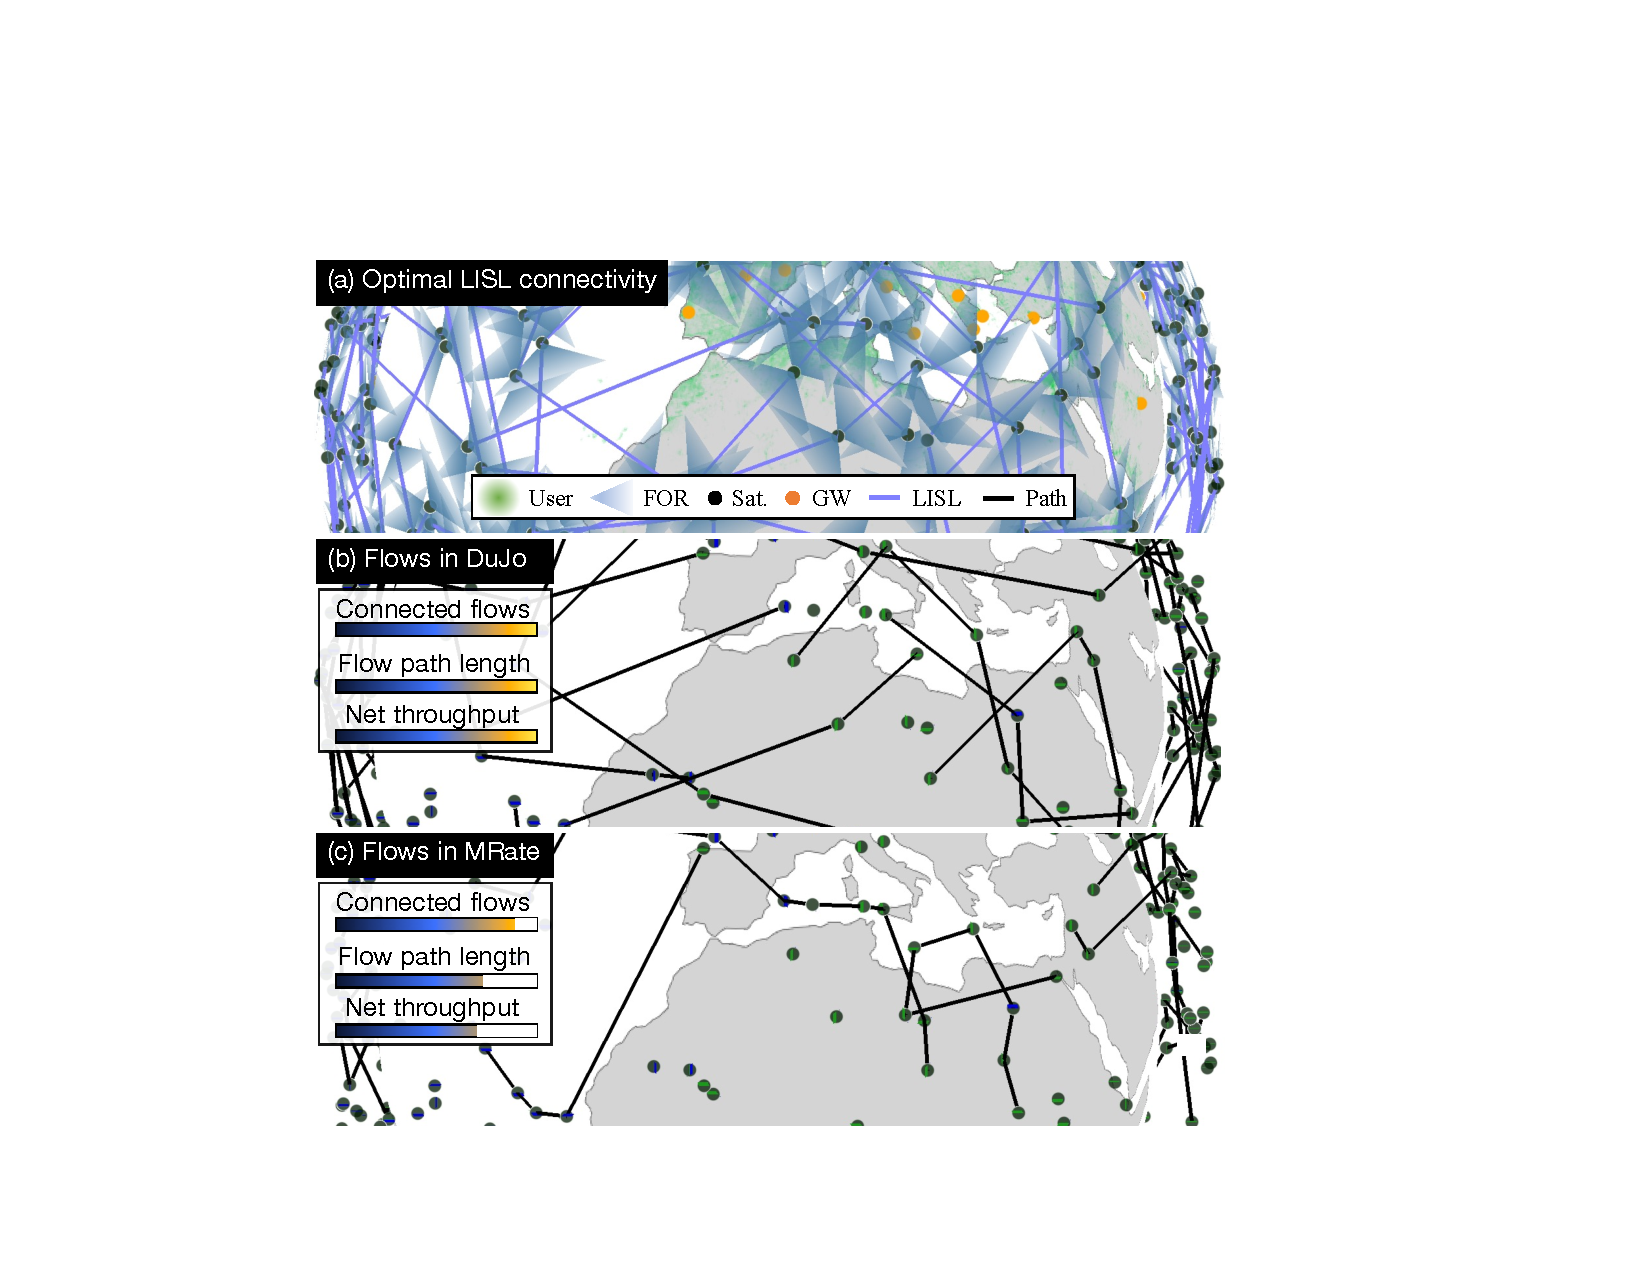
\includegraphics[width=.95\columnwidth]{constellation_simulation_1000_compare_rev.pdf}
  \caption{Constellations with $1000$ satellites randomly selected from the Starlink constellation: a) the constellation and LISLs connected in our DuJo scheme; b) and c) the comparison in the flow paths between our DuJo scheme and a non-joint scheme, MRate.}
  \label{fig:constellation_simulation_1000_compare}
\end{figure}

\section{Simulation Results}\label{sec:simulation}
\subsection{Simulation Setup}
To efficiently process the graphs and simulate the constellation, we implement our algorithms and simulations in a data-oriented programming paradigm. The constellation data is organized into contiguous data arrays and is processed in just-in-time (JIT) compiled procedures using Python Numba \cite{lam2015numba} for high computing efficiency. Linear programming is solved using the HiGHS solver \cite{huangfu2018parallelizing}. 
The simulations run on a workstation with an Intel Core Ultra 9 285K (24 cores) and 32 GB of memory.
\subsubsection{System Parameters}
We construct the constellation in simulations based on the real-world Starlink constellation TLE data from CelesTrak \cite{CelesTrak} at $\mathcal{T}_0$ as UTC $2025-07-16$ $16:00$. To simulate different constellation sizes, we randomly select $I$ satellites out of the Starlink constellation.
Each satellite has $N'=2$ LCTs: one LCT points in the direction of the satellite's velocity direction, and the other points in the opposite direction. The attitude control system maintains these orientations.
We configure the beam parameters as follows \cite{kaymak2018survey}: Each LCT has aperture area $A=0.01$ $\text{m}^2$ and responsivity $\Psi=0.5$ $\text{A/W}$. The noise current is $\sigma_{\mathrm{N}}=3\times 10^{-7}$~A in root-mean-square (RMS) value \cite{maxim_spf_transimpedance}.
The power of the beam is $P_0=20$ W and its bandwidth is $B=1$ GHz. The beam's wavelength is $1.55$ $\mu$m and the beam width is $100$ micro-radians, leading to the beam waist radius $W_0=9.87\times10^{-3}$ m and the Rayleigh range $z_\mathrm{R}=1.97\times10^{3}$ m \cite{saleh2019fundamentalsa}. 
The pointing jitter $\sigma_{\mathrm{J}}$ is set to $10$ micro-radians and the relaxed link outage probability $\epsilon$ is set to $0.001$.
The FOR of each LCT is within $\theta = 60$ degrees from its mounting direction and the maximum distance for two LCTs to establish a link is $\hat{z}=3000$ km.
The number $U_i$ of active users of each satellite $i$ depends on the real-world population data \cite{schiavina2023ghspop} under its coverage with approximately $200$ $\text{km}$ in radius. We assume that $0.01\%$ of the population is using the network at the given time, where $U_i$ is Poisson distributed with the mean population under satellite $i$'s coverage.
Each user will demand $D=0.1$ Gbps of data rate. We randomly select $100$ ground gateways locations around the globe from SatNOGS \cite{satnogs} to serve the traffic demand. We assume that each satellite can serve $Q=20$ Gbps traffic rate if there is a ground station in its coverage area.
If a satellite has positive traffic demand, it will try to route the traffic to the nearest $M=5$ satellites with ground stations connected, defining the traffic serving and demand pairs in $\mathcal{F}$.
Fig. \ref{fig:constellation_simulation_1000_compare} shows the constellations with $I=1000$, the uneven distribution of population density and ground gateway (GW) locations, emphasizing the need of considering these facts in our study.
It also compares the flow paths routed and the network throughput over the constellation between our DuJo scheme and a non-joint scheme (MRate as introduced below).
In the remaining simulation, we consider the constellation with $I=1000$ without explicit notation.

\begin{figure}[!t]
  \centering
  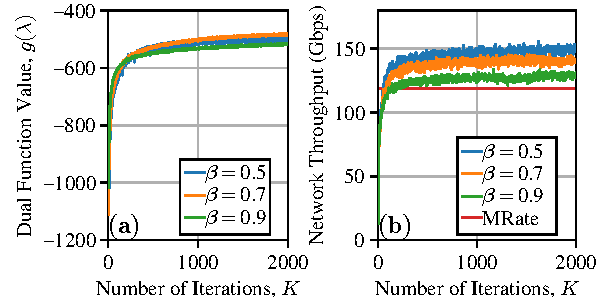
\includegraphics[scale=0.85]{plot_test_dual_optimization_starlink_constellation_varying_beta_d_o_and_p_o_horizontal.pdf}
  \caption{The convergence of our method, DuJo: a) the convergence of the subgradient descent, b) throughput using Lagrange multiplier conversion.}  \label{fig:plot_test_dual_optimization_starlink_constellation_varying_beta_d_o_and_p_o_horizontal}
\end{figure}
\subsubsection{Baseline Methods} 
We compare our duality-based joint method, with legend ``\textbf{DuJo}'', to the following baseline link matching and flow routing methods that make matching and routing decisions separately:
\begin{itemize}
    \item \textbf{+Grid:} A grid-based link matching \cite{bhattacherjee2019network} prioritizes the LCT pairs that are more aligned in their pointing directions, e.g., pairs with higher $\mathbf{d}_{i_n,i_m} \cdot \mathbf{u}_{m}+\mathbf{d}_{i_m,i_n} \cdot \mathbf{u}_{n}$.
    \item \textbf{Rand}: Random link matching randomly selects the LCT pairs to match, which is achieved by randomly setting the weights of LCT pairs and then applying the matching.
    \item \textbf{MRate:} Maximum link rate matching sets the weights of LCT pairs as their maximum transmission rates, $r_{n,m}$, as the objective is to maximize the network throughput.
    \item \textbf{OSPF:} For compared baselines, we use open shortest path first (OSPF) routing \cite{moy1998ospf} where the flows are routed using the link weights that are the reciprocal of aggregate rates of satellite pairs $1/\sum_{\{n,m\}\in \mathcal{E}_{i,j}} c_{n,m}r_{n,m}$.
\end{itemize}

\subsection{Numerical Results}
\subsubsection{Convergence of Dual Function}
The convergence of the dual function value $g(\lambda)$ is illustrated in Fig. \ref{fig:plot_test_dual_optimization_starlink_constellation_varying_beta_d_o_and_p_o_horizontal}a for different $\beta$ values. 
The results show that the dual function value increases and stabilizes over iterations, indicating convergence to the optimal value, as expected from Theorem \ref{theorem:convergence:classic}.
The performance of the converted LISL matching and flow routing decisions from the iterated Lagrange multipliers is shown in Fig. \ref{fig:plot_test_dual_optimization_starlink_constellation_varying_beta_d_o_and_p_o_horizontal}b.
The results show that the network throughput increases and stabilizes over iterations, indicating the optimized Lagrange multipliers lead to improved LISL matching and flow routing decisions. Also, the network throughput is higher in $\beta=0.5$ than the ones in $\beta=0.7$ and $0.9$, indicating that a slower step size decay rate leads to better performance due to more exploration of the Lagrange multipliers' space.
Also, we observe that the network throughput is achieving a near maximum value around $K=500$ iterations. For the remaining simulations, we fix $\beta=0.5$ and $K=500$.

\begin{figure}[!t]
  \centering
  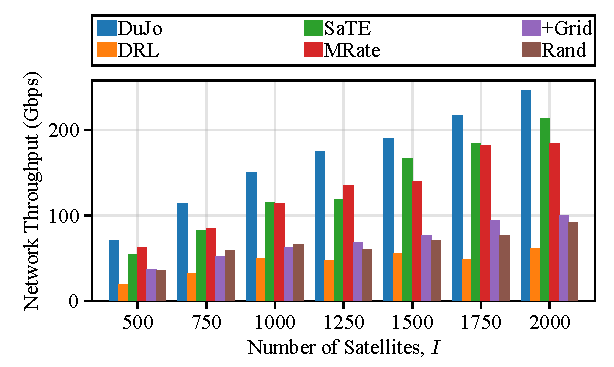
\includegraphics[scale=0.85]{plot_test_dual_optimization_vs_grid_rand.pdf}
  \caption{DuJo vs. baselines for different numbers of satellites $I$.}
  \label{fig:plot_test_dual_optimization_vs_grid_rand}
\end{figure}

\subsubsection{Comparison with Baselines}
We compare our method with the baseline methods in Fig. \ref{fig:plot_test_dual_optimization_vs_grid_rand}, where the network throughput is plotted against the number of satellites $I$ in the constellation.
The results show that our method improves the network throughput by approximately $35\%$$\sim$$145\%$, especially for larger constellations. Comparing with the grid-based and random methods, our method achieves a higher network throughput by around $145\%$. This is because our method considers the traffic flow rates and the LISL rates jointly, while the grid-based method only considers the pointing directions of the LCTs and the random method does not consider any information. When compared to the maximum link rate matching method, the outperformance is around $35\%$ for larger constellations, which is because our method optimizes the Lagrange multipliers to iteratively improve the LISL matching decisions based on the flow routing and the rate allocation, while the maximum link rate matching only considers the link rates and ignores the constellation connectivity.

\begin{figure}[t]
  \centering
  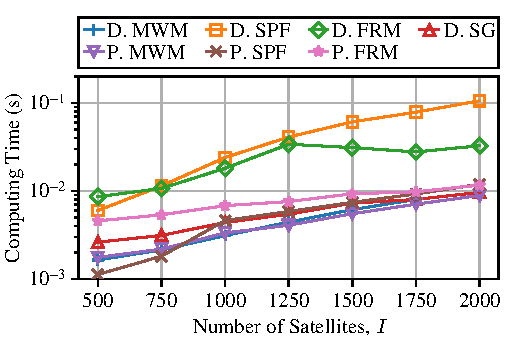
\includegraphics[scale=0.85]{plot_test_computing_time_measurement.pdf}
  \caption{Computing time measurement of steps in our method, DuJo, with legend as follows: steps of dual optimization: link matching \eqref{eq:routine:mwm_given_lambda}, flow routing \eqref{eq:routine:spf_given_lambda}, rate allocation \eqref{eq:routine:flow_rate_given_routing_cost}, subgradient descent step \eqref{eq:routine:dual_variable_update} (with legend ``D. MWM'', ``D. SPF'', ``D. FRM'' and ``D. SG'', respectively);
  steps of conversion of Lagrange multipliers: link matching with given Lagrange multipliers \eqref{eq:rounding:mwm}, flow routing with given matched LISLs \eqref{eq:rounding:spf} and rate allocation with matching and routing decisions \eqref{eq:rounding:frm} (with legend ``P. MWM'', ``P. SPF'' and ``P. FRM'').
  }
  \label{fig:plot_test_computing_time_measurement}
\end{figure}


\subsubsection{Evaluation of Computational Complexity}
We then evaluate the computational complexity of our method in Fig. \ref{fig:plot_test_computing_time_measurement} by measuring the computing time of the dual optimization algorithm in Algorithm \ref{alg:dual_optimization} and the conversion from Lagrange multipliers to the LISL matching and flow routing decisions in \eqref{eq:rounding:mwm}-\eqref{eq:rounding:frm}.
We observe that the computing time increases with the number of satellites $I$ in our method. Here, the conversion of the Lagrange multipliers can be done instantly within $1$ second.
The iterated steps in dual optimization can be achieved around $1$ second for each iteration. However, note that the algorithm needs a few hundred iterations to converge. This leads to a total computing time at the order of minutes for larger constellations, which requires further acceleration.



\subsubsection{Impact of Constellation Configurations}
We vary LCT configurations on each satellite, of which network throughput is shown in Fig. \ref{fig:plot_test_dual_optimization_vs_grid_rand_varying_availability_and_for}.
The results show that the network throughput increases with the average number of LCTs on each satellite. This is expected since more LCTs allow more LISLs to be established.
Our method consistently outperforms the baseline methods.
The maximum link rate matching method achieves the relatively higher network throughput with more LCTs. This is because high rate LISLs are more likely to be established when there are more LCTs.
Similarly, the network throughput increases when the FOR increases due to more options in the FOR. The performance of grid-based scheme is not varying much with the changing FOR, since only LCTs in the center of the steering range will be connected.
Next, we compare the performance of our method in different constellations. The results show that our method achieves the highest network throughput in all constellations, while the grid-based method achieves similar performance as ours in the walker-delta and OneWeb constellation. This is because the walker-delta and OneWeb constellations have highly regular satellite orbits, allowing the grid-based and maximum link rate matching methods to effectively establish those high-rate LISLs while maintaining the network connectivity for traffic flows.
However, in more complex constellations like Starlink, the grid-based method fails to exploit the high LISL rates in the not-well-aligned LCT pairs, and the maximum link rate matching method fails to establish the LISLs that are critical for the constellation connectivity.
On the other hand, our method can effectively exploit both link rates and constellation connectivity by optimizing the Lagrange multipliers iteratively, leading to the highest network throughput in all constellations.




\section{Conclusion}\label{sec:conclusion}
This paper proposed a Lagrangian duality-based method for joint link matching and traffic routing in satellite mega-constellations. The method applied the Lagrangian dual relaxation on per link rate limit constraints and decomposes the joint problem into easily solvable subproblems.
Simulations shown our method outperforms baseline methods in terms of network throughput in the constellation, which is achieved by optimizing the Lagrange multipliers iteratively to indicate the link's importance in connectivity as well as its rate congestion level, leading to better LISL matching and flow routing decisions.
It has also shown that the method can be practically computable given the NP-hardness of the original problem, while the computing time increases for larger constellations.
Research could be done to improve the computing efficiency, e.g., by learning to predict the Lagrange multipliers directly without iterations.
The observation on the LCT configurations' impact on the whole constellation suggests optimizing the LCT design to maximize the network profit.
Moreover, LISLs' acquisition and tracking processes can be investigated for their influence on the constellation throughput.

\begin{figure}[t]
  \centering
  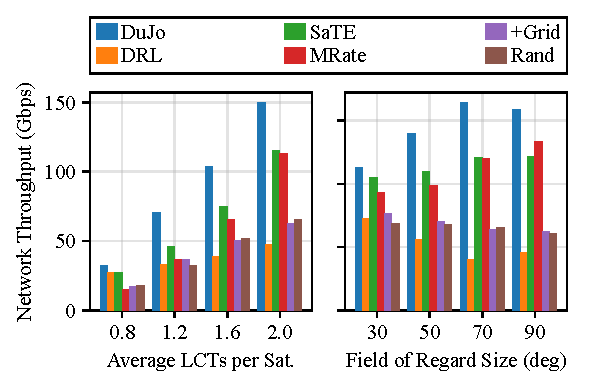
\includegraphics[scale=0.85]{plot_test_dual_optimization_vs_grid_rand_varying_availability_and_for.pdf}
  \caption{Comparison when varying LCT configurations on satellites.}
  \label{fig:plot_test_dual_optimization_vs_grid_rand_varying_availability_and_for}
\end{figure}

\begin{figure}[t]
  \centering
  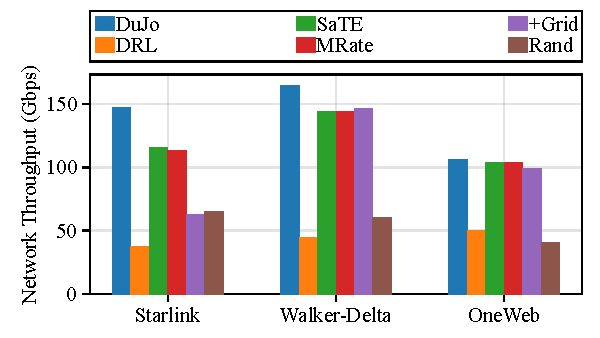
\includegraphics[scale=0.85]{plot_test_dual_optimization_different_constellation.pdf}
  \caption{Comparison in a Starlink-based ($I=1000$), a regular walker-delta ($50^{\circ}$ inclination, $I=1000$), and a OneWeb constellation ($I=650$).}
  \label{fig:plot_test_dual_optimization_different_constellation}
\end{figure}




% \appendix

\section*{Appendix: Proof of Lemma \ref{lemma:optimal_dual_variable_bounded}}
For given Lagrange multipliers $\lambda$, map them to new ones as $\lambda'_{i,j} = \min\{1, \lambda_{i,j}\}$, $\forall (i,j)\in\mathcal{L}$.
For $\lambda$, let the set of flows with routing cost greater than or equal to $1$ be $\mathcal{F}^+$ and those with routing cost less than $1$ as $\mathcal{F}^-$. Then, consider the flow costs for $\lambda'$. In the set $\mathcal{F}^-$, the routing cost is not changed since the routing cost was less than $1$ for $\lambda$ and is still the minimum cost for $\lambda'$.
In the set $\mathcal{F}^+$, assuming a flow's routing decisions are changed, and its cost becomes less than $1$, this new routing cost should be also the minimum cost for $\lambda$ since all links in the path have a cost less than $1$, which contradicts the fact that the minimum routing cost is greater than or equal to $1$ for flows in $\mathcal{F}^+$.
Therefore, the sets $\mathcal{F}^+$ and $\mathcal{F}^-$ remains the same for $\lambda'$ as for $\lambda$.
Since the flow rates of $\mathcal{F}^+$ computed in the dual function is always $0$ (due to the negative weights in the maximization objective) and the routing cost of flows in $\mathcal{F}^-$ remains the same, the value of the routing cost-weighted flow rate maximization is the same for $\lambda'$ and $\lambda$, i.e.,
\begin{equation}
  \begin{aligned}
      &\max_{
        \substack{
          \mathbf{q}\in \mathcal{Q}
        }
      }
      \big\{
      \sum_{(s,s')\in\mathcal{F} } q^{s,s'} (1 - \min_{
        \substack{
          \mathbf{x}^{s,s'}\in\mathcal{X}^{s,s'}
        }
      }
      \sum_{(i,j)\in\mathcal{L}}\lambda'_{i,j} x^{s,s'}_{i,j})   
      \big\}\\
      =
      &\max_{
        \substack{
          \mathbf{q}\in \mathcal{Q}
        }
      }
      \big\{
      \sum_{(s,s')\in\mathcal{F} } q^{s,s'} (1 - \min_{
        \substack{
          \mathbf{x}^{s,s'}\in\mathcal{X}^{s,s'}
        }
      }
      \sum_{(i,j)\in\mathcal{L}}\lambda_{i,j} x^{s,s'}_{i,j})   
      \big\}.
\end{aligned}
\notag
\end{equation}
Also, we have the MWM with $\lambda'$ leading to matched weights no greater than $\lambda$ since $\lambda'\leq\lambda$ as
\begin{equation}
  \begin{aligned}
&\max_{
  \substack{
    \mathbf{c}\in\mathcal{C}
  }
}
\big\{
\sum_{\{n,m\}\in\mathcal{E}} (\lambda'_{i_n,i_m} + \lambda'_{i_m,i_n})  r_{n,m} c_{n,m}
\big\}\\ 
\leq&
\max_{
  \substack{
    \mathbf{c}\in\mathcal{C}
  }
}
\big\{
\sum_{\{n,m\}\in\mathcal{E}} (\lambda_{i_n,i_m} + \lambda_{i_m,i_n})  r_{n,m} c_{n,m}
\big\}.
  \end{aligned}
  \notag
\end{equation}
Due to the above facts, $g(\lambda')\geq g(\lambda)$. Since we can always find such $\lambda'$ for any $\lambda$ as well as for any $\lambda^*$, there exist optimal Lagrange multipliers $\lambda^*$ with all elements less than or equal to $1$. Thus, the difference between $\lambda^{[1]}=\mathbf{0}$ and $\lambda^*$ can be bounded by $\|\mathbf{1}^{|\mathcal{E}|\times1}\|$. The boundedness of the maximum norm of the supergradient $\max_\lambda \|\delta(\lambda)\|$ is due to the fact that the traffic flow rates in $\mathcal{Q}$ are bounded and the capacities of LISLs are bounded by the maximum at zero distance.




\section*{Appendix: Proof of Theorem 1}
The Lagrange multipliers in the $k$-th iteration is denoted as $\lambda^{[k]}$. The optimal Lagrange multipliers are denoted as $\lambda^*$.
Denote the set of all possible supergradients of $g(\lambda^{[k]})$ at $\lambda^{[k]}$ as $\hat{\partial}_{\lambda^{[k]}} g(\lambda^{[k]}) \triangleq \{\delta| g(\lambda')\leq g(\lambda^{[k]}) + \delta^{\rm T}(\lambda'-\lambda^{[k]}), \forall \lambda'\}$.
$\delta(\lambda^{[k]})$ is a supergradient of $g(\lambda^{[k]})$ at $\lambda^{[k]}$, i.e., $ \delta(\lambda^{[k]}) \in \hat{\partial}_{\lambda^{[k]}}  g(\lambda^{[k]})$.
The difference between the optimal Lagrange multipliers $\lambda^*$ and the iterated ones $\lambda^{[k+1]}$ is given by
\begin{equation}
  \begin{aligned}
    &\|\lambda^{[k+1]} - \lambda^*\|^2 = \|\lambda^{[k]} + \alpha^{[k]} \delta(\lambda^{[k]}) - \lambda^*\|^2\\
  = &\|\lambda^{[k]} - \lambda^*\|^2 + 2\alpha^{[k]}\delta(\lambda^{[k]})^{\rm T} (\lambda^{[k]} - \lambda^*) + \|\alpha^{[k]}\delta(\lambda^{[k]})\|^2\\
\stackrel{\text{(a)}}{\leq}
    &\|\lambda^{[k]} - \lambda^*\|^2 + 2\alpha^{[k]} (g(\lambda^{[k]}) - g(\lambda^*)) + (\alpha^{[k]})^2 \|\delta(\lambda^{[k]})\|^2,
  \end{aligned}
  \notag
\end{equation}
where (a) is due to the definition of the supergradient. By applying telescoping sum, we have
\begin{equation}
  \begin{aligned}
    &\|\lambda^{[k+1]} - \lambda^*\|^2 \leq \|\lambda^{[1]} - \lambda^*\|^2 \\
    &+ 2 \sum_{i=1}^{k}\alpha^{[i]} (g(\lambda^{[i]}) - g(\lambda^*)) + \sum_{i=1}^{k}(\alpha^{[i]})^2 \|\delta(\lambda^{[i]})\|^2.
  \end{aligned}
  \notag
\end{equation}
Note that $g(\lambda^{[i]})\leq g(\hat{\lambda}^{[k]})$ $\forall i$ based on the definition of $\hat{\lambda}^{[k]}$, implying $\sum_{i=1}^{k}\alpha^{[i]} (g(\lambda^{[i]}) - g(\lambda^*)) \leq  \big(g(\hat{\lambda}^{[k]}) - g(\lambda^*)\big)\sum_{i=1}^{k}\alpha^{[i]}$.
Also, $\|\lambda^{[k+1]} - \lambda^*\|^2$ is non-negative. Substituting these facts in the above inequality, we have
\begin{equation}
  \begin{aligned}
    % &0\!\leq\! \|\lambda^{[1]} \!\!-\!\! \lambda^*\|^2 
    % \!+ \!2\! \sum_{i=1}^{k}\alpha^{[i]} (g(\lambda^{[i]})\! -\! g(\lambda^*)) \!+\! \sum_{i=1}^{k}(\alpha^{[i]})^2 \|\delta(\lambda^{[i]})\|^2\\
    % &\Rightarrow\sum_{i=1}^{k}\alpha^{[i]} (g(\lambda^*) - g(\hat{\lambda}^{[k]}))\\
    % &\qquad\qquad \leq \frac{\|\lambda^{[1]} - \lambda^*\|^2+\sum_{i=1}^{k}(\alpha^{[i]})^2 \|\delta(\lambda^{[i]})\|^2}{2} \Rightarrow \\
    &g(\lambda^*) - g(\hat{\lambda}^{[k]}) \leq \frac{\|\lambda^{[1]} - \lambda^*\|^2+\sum_{i=1}^{k}(\alpha^{[i]})^2 \|\delta(\lambda^{[i]})\|^2}{2\sum_{i=1}^{k}\alpha^{[i]}}.
  \end{aligned}
  \notag
\end{equation}
Using the convergence of $\sum_{i=1}^{k}\alpha^{[i]}$ and $\sum_{i=1}^{k}(\alpha^{[i]})^2$ when $0.5\leq \beta < 1$ \cite{boyd2003subgradient} and the boundedness of $\|\lambda^{[1]} - \lambda^*\|^2$ and $\max_\lambda \|\delta(\lambda)\| $ from Lemma \ref{lemma:optimal_dual_variable_bounded}, we prove the statement.

\bibliography{main}
\bibliographystyle{IEEEtran}

\end{document}